\documentclass[spanish]{article}
\usepackage{graphicx}
\usepackage{ragged2e}
\usepackage{geometry}
\usepackage{float}
\usepackage[table,xcdraw]{xcolor}
\title {Práctica 1: Determinación experimental de la complejidad de un algoritmo}
\graphicspath{{../img/}}
\addtolength{\textheight}{1.5in} 
\begin{document}
	\centerline{
\includegraphics[width=450px,height=100px]{header}}
	\centerline{Analisis de algoritmos, Sem: 2021-1, 3CV1,Práctica  2, 27/10/2020}
	\centering{\huge{Práctica 2: Funciones Recursivas vs Iterativas}}
	\centerline{\newline{\textbf{Bejar Valencia Angel Ivan,Payán Téllez René}}}
	\newline{\textit{ivanbejar07@gmail.com,rpayant1500@alumno.ipn.mx}}
	\bigskip
	\justify
	\textbf{Resumen:}	
	En esta practica se compararan la complejidad de los algorimos iterativos y recursivos
	\textbf{Palabras clave:}
	Iterativo,Complejidad,Recursivo,C/C++
	\section{Introduccion}
	Durante esta práctica, se analizará y comparará la complejidad de soluciones iterativas y recursivas para el mismo algoritmo. La diferencia entre una solución iterativa y una solución recursiva es que, en una solución recursiva, se invoca la respuesta de múltiples invocaciones de la misma función, para obtener una respuesta a partir de la división del problema en partes mas pequeñas. Mientras que, en una solución iterativa, no se hace uso de dicho recurso, todo el algoritmo se ejecuta sin necesidad de invocar a una función desde sí misma. Por lo que se pueden realizar soluciones al mismo problema de ambas formas y estas a su vez podrian tener distintas complejidades.
	\section{Conceptos Basicos}
	\subsection{Algoritmo}
	La palabra algoritmo proviene del sobrenombre de un matemático árabe del siglo IX, Al-Khwarizmi, que fue reconocido por enunciar paso a paso las reglas para las operaciones matemáticas básicas con decimales (suma, resta, multiplicación y división).	
	Vemos definición de algoritmo como un grupo de órdenes consecutivas que presentan una solución a un problema o tarea. Algunos ejemplos de algoritmos los podemos encontrar en las matemáticas (como el algoritmo para resolver una multiplicación) y en los manuales de usuario de un aparato (como una lavadora o una impresora).	
	Sin embargo, hoy en día se relaciona la palabra algoritmo con el mundo de la informática, más concretamente en la programación; los conocidos como algoritmos informáticos.[1]
	\subsection{Complejidad algoritmica}
	Así que, por su naturaleza, un problema tiene la capacidad de ser solucionado por uno o varios métodos, pero si bien es importante llegar a la respuesta, más importante es evaluar su viabilidad. Siempre que se analiza y evalúa adecuadamente la efectividad de una solución, disminuye drásticamente el costo que representa su producción y mantenimiento, pues los recursos que se invierten posteriormente en codificación, pruebas y revisión es mucho menor siempre (como el tiempo, dinero y talento humano).	
	Entrando en materia, la complejidad algorítmica es una métrica teórica que nos ayuda a describir el comportamiento de un algoritmo en términos de tiempo de ejecución (tiempo que tarda un algoritmo en resolver un problema) y memoria requerida (cantidad de memoria necesaria para procesar las instrucciones que solucionan dicho problema). Esto nos ayuda a comparar entre la efectividad de un algoritmo y otro, y decidir cuál es el que nos conviene implementar.[2]
	\subsection{Algoritmo Iterativo}
	Las instrucciones de repetición, de iteración o bucles, facilitan la repetición de un bloque de instrucciones, un número determinado de veces o mientras se cumpla una condición.	
	Por lo general, existen dos tipos de estructuras iterativas o bucles en los lenguajes de programación. Encontraremos un tipo de bucle que se ejecuta un número preestablecido de veces, que es controlado por un contador o índice, incrementado en cada iteración. Este tipo de bucle forma parte de la familia for.	
	Por otro lado, encontraremos un tipo de bucle que se ejecuta mientras se cumple una condición. Esta condición se comprueba al principio o el final de la construcción. Esta variante pertenece a la familia while or repeat, respectivamente.[2]
	\subsection{Algoritmo Recursivo}
	Los algoritmos   recursivos   se   basan   en   la   metodología   de   llamar   repetidamente  la  propia  función  en  que  están  definidos,  y  son  de  gran  utilidad  en  multitud de campos en la informática.[3]\\
	La solución de un algoritmo recursivo comienza a atacar un problema tomando un problema grande y lo va dividiendo hasta llegar a problemas más pequeños que son sencillos o triviales de resolver. Una vez que llega a estos problemas más pequeños, vuelve por donde llegó y comienza a combinar las soluciones entre si para obtener la solución al problema más grande.[4]
	\section{Experimentacion y Resultados}
		\subsection{Producto}
			De la primer seccion de problemas se decidio iterar sobre todos los n y m posibles desde 0 hasta 1000.\\
			\begin{figure}[h!]
				\centering
				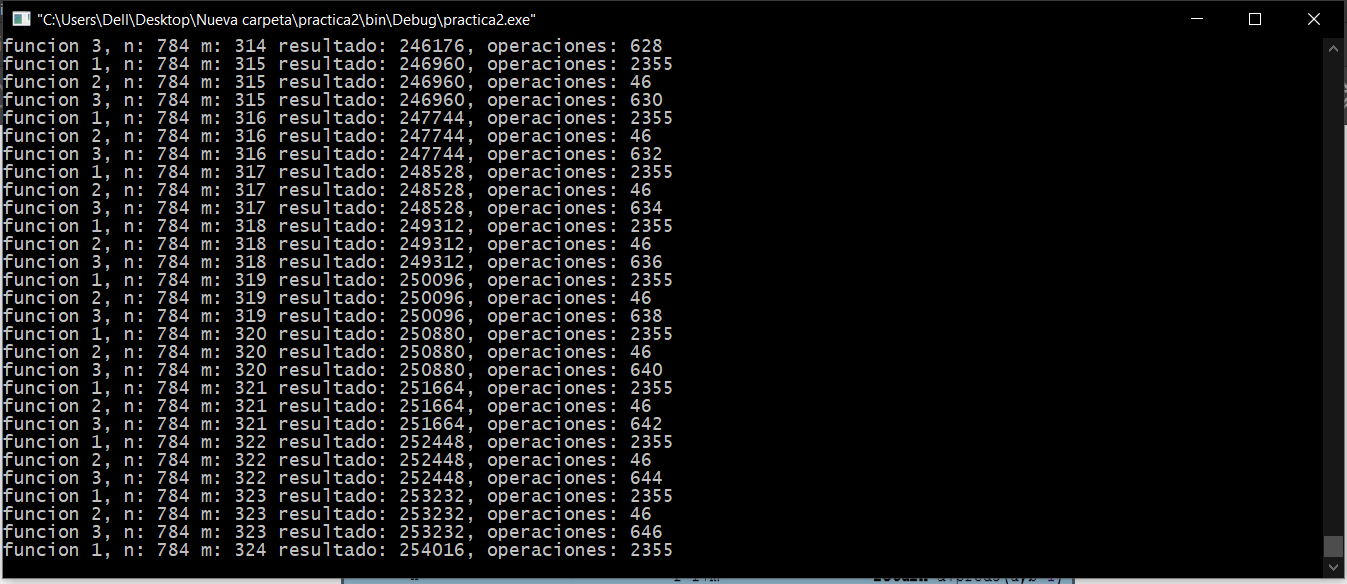
\includegraphics[width=400px,height=200px]{ejecucionPrimeraParte}
				\caption{Ejecucion del programa que contiene las tres primeras funciones}
			\end{figure}
			\begin{figure}[h!]
				\centering
				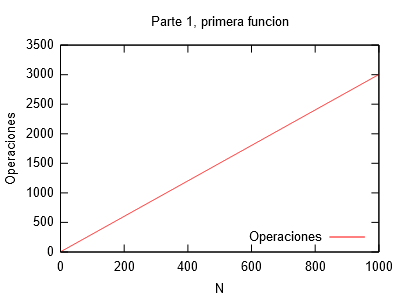
\includegraphics[width=400px,height=300px]{grafica1}
				\caption{N contra Operaciones de la primer funcion}
			\end{figure}
			\begin{figure}[H]
				\centering
				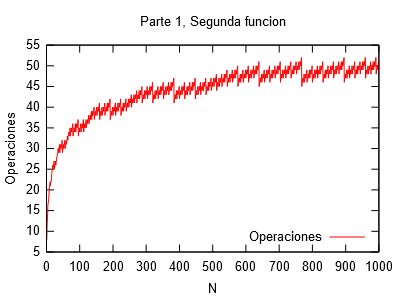
\includegraphics[width=400px,height=300px]{grafica2}
				\caption{N contra Operaciones de la segunda funcion}
			\end{figure}
			\begin{figure}[H]
				\centering
				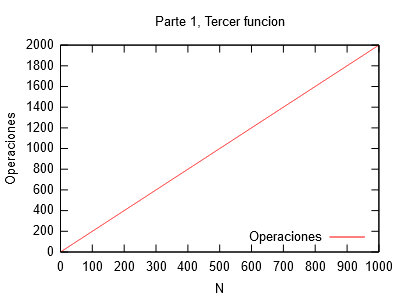
\includegraphics[width=400px,height=300px]{grafica3}
				\caption{N contra Operaciones de la tercer funcion}
			\end{figure}
			\begin{figure}[H]
				\centering
				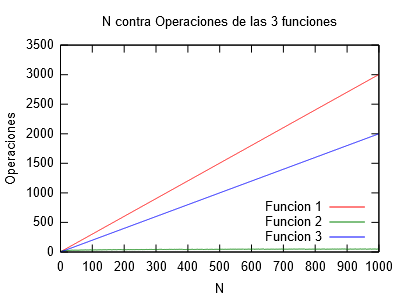
\includegraphics[width=400px,height=300px]{grafica4}
				\caption{N contra Operaciones de las 3 funciones combinadas}
			\end{figure}
			Al terminar se determino que el número de operaciones solo se ve afectado por "n", no por "m", por lo que se decidio graficar solo dichos valores.\\
			Tambien podemos observar que de las 3 funciones, la función número 2 es la mas optima y la numero 1 la menos optima.\\
			De forma Experimental podemos concluir lo siguiente:
			\begin{table}[H]
				\begin{tabular}{|l|l|l|l|}
					\hline
					\rowcolor[HTML]{FFFE65} 
					\multicolumn{1}{|c|}{\cellcolor[HTML]{FFFE65}{\color[HTML]{000000} \textbf{Funcion}}} & \multicolumn{1}{c|}{\cellcolor[HTML]{FFFE65}{\color[HTML]{000000} \textbf{Peor escenario}}} & \multicolumn{1}{c|}{\cellcolor[HTML]{FFFE65}{\color[HTML]{000000} \textbf{Mejor escenario}}} & \multicolumn{1}{c|}{\cellcolor[HTML]{FFFE65}{\color[HTML]{000000} \textbf{Orden de complejidad}}} \\ \hline
					1                                                                                     & n\textgreater{}0                                                                            & $n=0$                                                                                          & $O(3*n)                                                                                           $ \\ \hline
					2                                                                                     & n\textgreater{}0 y n\%2!=0                                                                  & $n=0$                                                                                          & $O(5log_2(n+1))$                                                                                   \\ \hline
					3                                                                                     & n=0 (Nunca termina), n\textgreater{}1 para todo lo demas                                    & $n=1$                                                                                          & $O(2*n)$                                                                                            \\ \hline					
				\end{tabular}
				\caption{Resultados obtenidos a partir del analisis a posteriori}
			\end{table}
		\subsection{Cociente}
		\section{Conclusiones}
		\section{Anexo}
			\subsection{Producto}
				\subsection*{Función 1}
					De esta función podemos analizar que su peor escenario es cuando: $n>0$, ya que a partir de este punto se comportara de forma lineal. Mientras que su mejor escenario es cuando $n=0$.\\
					Posteriormente se realizo el analisis a priori:\\
					\begin{center}
						\begin{table}[H]
							\begin{tabular}{|l|l|l|}
								\hline
								\rowcolor[HTML]{FFCC67} 
								Codigo                           & Costo & Veces ejecutado \\ \hline
								\textit{r = 0}                    & $C_1$    & 1               \\ \hline
								\textit{while(n\textgreater{}0)} & $C_2$    & n+1             \\ \hline
								\textit{\  \  r = r+m}                 & $C_3$    & n               \\ \hline
								\textit{\  \  n--}                     & $C_4$    & n               \\ \hline
								\textit{return r}                & $C_5$    & 1               \\ \hline
							\end{tabular}
						\end{table}						
							$T(n) = C_1+(n+1)C_2+n(C_3+C_4)+C_5$\\							
							$T(n) = n(C_2+C_3+C_4)+C_1+C_2+C_5$\\							
							$T(n) \in \Omega(1)$\\							
							$T(n) \in \O(n)$\\
					\end{center}
				\subsection*{Función 2}
					De esta función podemos analizar que su peor escenario es cuando: $n>0$ y $n$ no sea par (ejecuta el ciclo una vez mas), ya que a partir de este punto se comportara de forma logaritmica. Mientras que su mejor escenario es cuando $n=0$.\\
					Posteriormente se realizo el analisis a priori:\\
					\begin{center}
							\begin{table}[H]
								\begin{tabular}{|l|l|l|}
									\hline
									\rowcolor[HTML]{FFCC67} 
									Codigo                           & Costo & Veces ejecutado \\ \hline
									\textit{r =0}                    & $C_1$    & 1               \\ \hline
									\textit{while(n\textgreater{}0)} & $C_2$    & $log_2(n)+1$       \\ \hline
									\textit{\  \  if(n \& 1)}              & $C_3$    & $log_2(n)$         \\ \hline
									\textit{\  \  \  \  r = r+m}                 & $C_4$    & $log_2(n)/2$       \\ \hline
									\textit{\  \  m=2*m}                            & $C_5$    & $log_2(n)$         \\ \hline
									\textit{\  \  n=n/2}                            & $C_6$    & $log_2(n)$         \\ \hline
									\textit{return r}                & $C_7$    & 1               \\ \hline
								\end{tabular}
							\end{table}
								$T(n) = C_1 + C_2(log_2(n)+1) + C_4(\frac{log_2(n)}{2}) + log_2(n)(C_5+C_6+C_3) + C_7$
								$T(n) = log_2(C_2+C_5+C_6+C_7) + C_4\frac{log_2(n)}{2} + C_1 + C_7$
								$T(n) = log_2(C_2+\frac{C_4}{2}+C_5+C_6+C_7) + C_1 + C_7$\\
								$T(n) \in \Omega(1)$\\
								$T(n) \in \O(log_2(n))$
					\end{center}
				\subsection*{Función 3}
					De esta función podemos analizar que su peor escenario es cuando: $n>1$, ya que a partir de este punto se comportara de forma lineal. Mientras que su mejor escenario es cuando $n=1$.\\
					\textbf{Nota: debido a la forma de la implementacion cuando n $<$ 1 el algoritmo no termina}
					Posteriormente se realizo el analisis a priori:\\
					\begin{center}
						\begin{table}[H]
							\begin{tabular}{|l|l|l|}
								\hline
								\rowcolor[HTML]{FFCC67} 
								Codigo                               & Costo & Veces ejecutado \\ \hline
								\textit{if b == 1}                   & $C_1$   & n               \\ \hline
								\textit{\  \  return 1}              & $C_2$   & 1               \\ \hline
								\textit{else}                        & 0     &                 \\ \hline
								\textit{\  \  return a+prod3(a,b-1)} & $C_4$   & n-1             \\ \hline
							\end{tabular}
						\end{table}
						$T(n) = C_1(n) + C_2 + C_3(n-1)$\\
						$T(n) = n(C_1+C_3) + C_2 - C_3$\\
						$T(n) \in \Omega(1)$\\
						$T(n) \in \O(n)$
					\end{center}
				\subsection*{Comparacion}
				Despues de obtener la complejidad a priori y a posteriori de las 3 funciones, se concluye que la funcion 2 es la mas optima y el algoritmo número 1 es el menos optimo.
				% Please add the following required packages to your document preamble:
				% \usepackage[table,xcdraw]{xcolor}
				% If you use beamer only pass "xcolor=table" option, i.e. \documentclass[xcolor=table]{beamer}
				\begin{table}[H]
					\begin{tabular}{|l|l|l|}
						\hline
						\rowcolor[HTML]{FFCC67} 
						Funcion & Calculo a priori & Calculo a posteriori \\ \hline
						\rowcolor[HTML]{FE0000} 
						1       & $O(n)$           & $O(3n)$              \\ \hline
						\rowcolor[HTML]{32CB00} 
						2       & $O(log_2(n))$    & $O(5log_2(n+1))$     \\ \hline
						\rowcolor[HTML]{F8FF00} 
						3       & $O(n)$           & $O(2n)$              \\ \hline
					\end{tabular}
				\end{table}
			\subsection*{Cociente}
		\section{Bibliografia}

\end{document}